\chapter{Experiments\label{cha:chapter5}}
The chapter provides a detailed analysis of the models proposed in \autoref{cha:chapter4}. It also introduces a novel loss function, \ac{dualmse} loss, as well as a training procedure optimized for the \ac{mymodel} architecture. All learning-based compression methods explored in this thesis use a set of hyper-parameters to determine different aspects of the model and its training process. Most of these hyper-parameters are specific to a model or an experiment and are therefore noted in the experiments they employed in. However, some hyper-parameters are equal for all experiments. In all experiments, the chosen optimizer is the Adam optimizer with $\beta_1=0.9$ and $\beta_2=0.999$. The learning rate is set to $0.5 \cdot 10^{-5}$ for most experiments. If a different learning rate is used for an experiment, it is noted explicitly.

\section{Description of the Dataset\label{sec:dataset}}
The dataset used in this thesis is the HySpecNet-11k dataset proposed by Fuchs et al. \citep{fuchs_hyspecnet-11k_2023}. HySpecNet-11k is a hyperspectral benchmark dataset that consists of 11,483 image patches containing large-scale views of the surface of the earth. The patches were obtained from image tiles from the \ac{enmap} satellite mission \citep{guanter_enmap_2015}. The image patches do not overlap which is advantageous for use in learning-based approaches as there are no duplicated image parts in the training set. The source data for the dataset uses 224 spectral bands and $128\times 128$ pixels spatially with a \ac{gsd} of 30 meters. However, we use the preprocessed version of the dataset which removes spectral bands due to high water vapor absorption in those bands. We therefore only use 202 spectral bands. The image patches are of high quality because the tiles they were obtained from contain less than 10\% snow and cloud cover and were radiometrically, geometrically and atmospherically corrected \citep{fuchs_hyspecnet-11k_2023}. Furthermore, cropped patches at the borders of tiles were discarded, so each image patch contains information in all $128\times 128$ pixels. For splitting the dataset into training, validation and test sets we used the provided patch-wise splitting set. In this splitting set patches from the same tile can be present in different sets, unlike in the tile-wise splitting set. We did not perform experiments with the tile-wise splitting set as it is outside of the scope of this thesis. It is however a potential future research direction.

\section{Loss Functions and Metrics}
We use three different loss functions for the models in this thesis. Some models use the \ac{mse} loss function, which is commonly used in the domain of machine learning. However, to optimize the training process for the \ac{mymodel} architecture, we developed a novel loss function based on \ac{mse} loss named \ac{dualmse} loss for these models. In addition to this, the hyperprior-based models are designed to be trained using a \acf{rd} loss function which allows for changing the target bitrate by varying a hyperparameter.
\subsection{MSE Loss}
The \ac{mse} function is a common loss function used for training \acp{ann}. For the task of compressing a hyperspectral image it can be defined as follows:
\begin{align}
\text{MSE}(X,\hat{X}) = \frac{1}{B\cdot C\cdot H\cdot W} \sum_{b=1}^{B}\sum_{c=1}^{C}\sum_{h=1}^H\sum_{w=1}^W (x_{bchw} - \hat{x}_{bchw})^2
\end{align}
Here $X$ is defined as a batch of hyperspectral input images, $\hat{X}$ the reconstruction of the images in $X$ obtained from the compression model, $B$ the number of images per batch and $C$,$H$ and $W$ the number of spectral channels, height and width of the hyperspectral images respectively.
We use \ac{mse} loss for pre-training the spectral autoencoder models as well as for training the \ac{cnn}-based spatial autoencoder outside of \ac{mymodel}.

\subsection{Rate Distortion Loss\label{sec:ch5ratedistortion}}
In contrast to the purely \ac{cnn}-based models with a fixed compression rate for a given set of hyper-parameters, the hyperprior-based models have a variable compression rate that changes during the training process. This comes from the fact that the bitrate of the arithmetic coder depends on the performance of the hyperprior \ac{cnn}. Because of this \ac{mse} loss is not optimal for these models. While it is possible to train hyperprior-based models using \ac{mse} loss because the bitrate dependency is contained in the lossless arithmetic coder, this leads to very high bitrates. However, using \ac{mse} loss for a hyperprior model can still be useful to obtain an upper bound on the reconstruction accuracy for a given set of hyper-parameters. For more elaboration on this see \autoref{sec:ch5hyperprior}.

To train a model using an arithmetic coder in the bottleneck with both a low distortion and a low bitrate, a different loss function is needed. The type of problem that arises is a rate-distortion optimization problem \citep{balle_variational_2018}. This problem can be parametrized in the following way \citep{minnen_joint_2018}:
\begin{align}
L_{RD} = R + \varphi \cdot D = \underbrace{\mathbf{E}_{x\sim p_x} [ -\log_2 p_{\hat{y}}(\lfloor f(x)\rceil)]}_\text{rate}+ \underbrace{\varphi \cdot\mathbf{E}_{x\sim p_x} [d(x,g(\lfloor f(x)\rceil))]}_\text{distortion}.
\end{align}
We parametrize the rate-distortion trade-off with the Lagrange multiplier $\varphi$. (We use $\varphi$ instead of the commonly used $\lambda$ to avoid confusion with the $\lambda$ of the \ac{dualmse} loss described in \autoref{sec:ch5dualmse}). $p_x$ is the unknown distribution of input images, $\lfloor\cdot\rceil$ refers to quantization and $f$ is the main encoder. Accordingly, $y=f(x)$ is the output of the main encoder applied to the input $x$, $\hat{y} = \lfloor y\rceil$ are the quantized latents of the main encoder, $p_{\hat{y}}$ is a discrete entropy model and $\hat{x}=g(\hat{y})$ is the reconstruction of $x$ obtained from applying the main decoder $g$ to the quantized latents $\hat{y}$. As the metric for computing the distortion, we use \ac{mse}, because Ballé et al. showed that the rate-distortion problem is equivalent to minimizing the \ac{kl} divergence over $p_x$ \citep{balle_variational_2018}. Using this equivalence they showed that using \ac{mse} as the distortion metric is equivalent to assuming a Gaussian distribution for $p_{x|\hat{y}}(x|\hat{y})$. While there are approaches assuming different probability distributions like the Student's T distribution, this was not a focus of this thesis and the Gaussian often provides a good estimate for unknown probability distributions. For this reason, we also assumed a Gaussian distribution for the probability distribution.

However, this formulation does not include the hyperprior network that learns and transmits side information about the entropy model $p_{\hat{y}}$. In order to incorporate the hyperprior into the \ac{rd} loss function, we need to add an additional term to capture the bitrate for the transmitted side information. The final loss function is then defined as follows:
\begin{align}
L_{RD}=R + \varphi \cdot D &= \underbrace{\mathbf{E}_{x\sim p_x} [ -\log_2 p_{\hat{y}}(\lfloor f(x)\rceil)]}_\text{rate (main latents)} + 
\underbrace{\mathbf{E}_{x\sim p_x} [ -\log_2 p_{\hat{z}}(\lfloor f_h(f(x))\rceil)]}_\text{rate (hyper-latents)} \nonumber\\
&\qquad\qquad\qquad\qquad\qquad\quad\:\: + \underbrace{\varphi \cdot\mathbf{E}_{x\sim p_x} [\Vert x - g(\lfloor f(x)\rceil))\Vert^2_2]}_\text{distortion}.\nonumber\\
&=\underbrace{\mathbf{E}_{x\sim p_x} [ -\log_2 p_{\hat{y}}(\hat{y})]}_\text{rate (main latents)} + 
\underbrace{\mathbf{E}_{x\sim p_x} [ -\log_2 p_{\hat{z}}(\hat{z})]}_\text{rate (hyper-latents)} + \underbrace{\varphi \cdot\mathbf{E}_{x\sim p_x} [\Vert x - \hat{x}\Vert^2_2]}_\text{distortion}
\end{align}
Here $z$ and $\hat{z}$ refer to the latent of the hyperprior and the quantized latent of the hyperprior respectively, that is the result of applying both the main encoder $f$ and the hyperprior encoder $f_h$ to the input $x$.

It is to note, that since only the distortion metric is dependent on $\varphi$, \ac{rd} loss converges to that metric for $\varphi\rightarrow\infty$ if we assume an appropriately scaled learning rate. Since we use \ac{mse} loss for the distortion metric, for our experiments \ac{rd} loss converges to \ac{mse} loss for $\varphi\rightarrow\infty$.

With regard to the quantization operation, care has to be taken. When executing the trained hyperprior model, quantization is defined as rounding to the nearest integer. However, during training, this would result in zero gradients everywhere. To avoid this, while training we instead apply a uniform noise to the input in place of rounding. From this follows that the arithmetic coder is only executed during testing, not during training. In training the achieved bitrate is estimated using a heuristic. However, we verified that the bitrate estimates are close to the real achieved bitrate in \autoref{sec:ch5heur}.
\subsection{Dual MSE Loss}
\ac{mymodel} consists of an outer autoencoder model and an inner autoencoder model. However, applying a loss function such as \ac{mse} loss in the standard way results in the inner autoencoder being trained through a layer of distortion at both the input and the output, as the input to the loss function is the input to outer encoder $x$ and the output of the outer decoder $\hat{x}$. The input to the inner encoder, $y=f_o(x)$, where $f_o$ is the outer encoder and the output of the inner decoder, $\hat{y}=g_i(f_i(y))$, where $f_i$ and $g_i$ are the inner encoder and decoder respectively, are not direct inputs to the loss functions. To alleviate that, we designed an experimental loss function called \ac{dualmse} loss. It is defined as follows:
\begin{align}
\text{DualMSE}(x,\hat{x},y,\hat{y}) = \lambda \cdot \text{MSE}(x,\hat{x}) + (1-\lambda) \cdot  \text{MSE}(y,\hat{y}).
\end{align}
The \ac{dualmse} loss is therefore a linear interpolation between the \ac{mse} loss of the complete model and the \ac{mse} loss of the inner model. This allows for fine-grained control over the weight of the loss of the inner model in the overall loss. Of note are also the two edge cases of $\lambda = 1$, where the \ac{dualmse} loss function becomes equivalent to \ac{mse} loss and $\lambda = 0$, where only the loss of the inner model is used. The \ac{dualmse} loss was used for \ac{mymodel} models using the \ac{cnn}-based spatial autoencoder. Results regarding the use of \ac{dualmse} loss for these models can be seen in \autoref{sec:ch5dualmse}. While the use of a Dual Rate-Distortion loss would be possible for \ac{mymodel} using a hyperprior-based spatial autoencoder, this was not done because the results in \autoref{sec:ch5dualmse} did not show a clear and significant improvement when using a dual loss function.

\subsection{Metrics}
\begin{table}
\centering
\caption[Acronyms for Commonly Used Models]{Acronyms for commonly used models in this section.}
\begin{tabularx}{\textwidth}{|L|L|}
\hline
Model Name & Description \\
\hline\hline
Conv1D & Per-pixel spectral autoencoder (\autoref{sec:conv1d})\\
\hline
FastConv1D & \Ac{twod} spectral autoencoder (\autoref{sec:fastconv1d})\\
\hline
Conv2D & \Ac{twod} \ac{cnn}-based spatial autoencoder (\autoref{sec:conv2d})\\
\hline
AttentionHyperprior & Attention-based spatial model using hyperprior architecture (\autoref{sec:atthyperprior}) \\
\hline
\ac{mymodel} & \ac{mymodel} using Conv1D as the spectral part and Conv2D as spatial part (\autoref{sec:combinedmodel}) \\
\hline
\ac{mymodel}-Fast & \ac{mymodel} using FastConv1D as the spectral part and Conv2D as spatial part (\autoref{sec:combinedmodel}) \\
\hline
\ac{mymodel}-Attention & \ac{mymodel} using Conv1D as the spectral part and AttentionHyperprior as spatial part (\autoref{sec:combinedmodel}) \\
\hline
Spectral-VAE & Spectral \ac{vae}-based autoencoder (\autoref{sec:vae}) \\
\hline
\end{tabularx}
\label{fig:shortnames}
\end{table}
We use two different metrics to evaluate our experiments. The first metric is \ac{psnr}, which is a common metric to quantify reconstruction accuracy for lossy learning-based image compression \citep{balle_end--end_2017,balle_variational_2018,minnen_joint_2018,kuester_1d-convolutional_2021,kuester_transferability_2022,la_grassa_hyperspectral_2022}. \Ac{psnr}  is defined in general as follows:
\begin{align}
\text{PSNR}(x,\hat{x}) &= 10\cdot \log_{10}\frac{\text{MAX}}{\text{MSE}(x,\hat{x})}
&= 20 \cdot \log_{10}(\text{MAX}) - 10\cdot \log_{10}(\text{MSE}(x,\hat{x})).
\end{align}
Here MAX is the maximum possible pixel value in the used dataset and $\text{MSE}(x,\hat{x})$ refers to the Mean Squared Error between $x$ and $\hat{x}$. However, since the data range for the HySpecNet-11k dataset used in this thesis is the interval $[0,1]$, the equation simplifies to:
\begin{align}
\text{PSNR}(x,\hat{x}) = - 10\cdot \log_{10}(\text{MSE}(x,\hat{x})).
\end{align}
It is therefore directly correlated with the log of the \ac{mse}.
While \ac{psnr} is a commonly used metric in lossy learning-based hyperspectral compression, it is computed as an average over all channels. We therefore want to employ another metric to more accurately evaluate the reconstruction of the spectral signatures which are important for lossy reconstructions of hyperspectral images.

For this, we use the spectral angle. It is computed by calculating the angle between the spectra of the input image and the reconstruction for each pixel using the \ac{sam} algorithm \citep{kruse_spectral_1993}. The computed angles are then averaged to compute the metric for a given input image and reconstruction. Using the combination of \ac{psnr} and spectral angle we can compare different models with regard to spatial and spectral reconstruction accuracy.
\section{Impact of Hughes Phenomenon \label{sec:ch5hughes}}
\begin{figure}[!ht]
    \centering
\pgfplotstableread[col sep=semicolon,]{graphs/hughes.csv}\datatable
\begin{tikzpicture}
\begin{semilogxaxis}[
	log ticks with fixed point,
	grid=both,
    width=\textwidth,
    height=10cm,
    xtick=data,
    xticklabels from table={\datatable}{dspercent},
    legend style={at={(0.98,0.3)},anchor=south east},
    ylabel={PSNR (dB)},
    xlabel={Fraction of dataset used (\%)}]
    
    \addplot [mark=o, blue!80 ] table [x={dspercent}, y={fastconv_psnr}]{\datatable};
    \addlegendentry{FastConv}
    
    \addplot [mark=o, red!80] table [x={dspercent}, y={fastcombined_psnr}]{\datatable};
    \addlegendentry{\ac{mymodel}-Fast}
\end{semilogxaxis}
\end{tikzpicture}
\caption[Comparison for Different Dataset Sizes (PSNR)]{PSNR for the model FastConv and \ac{mymodel}-Fast for different subsections of the dataset. Only training and validation set sizes were reduced, and all models were evaluated on the full test set.}
\label{fig:hughes}
\end{figure}

\begin{figure}[!ht]
    \centering
\pgfplotstableread[col sep=semicolon,]{graphs/hughes.csv}\datatable
\begin{tikzpicture}
\begin{semilogxaxis}[
	log ticks with fixed point,
	grid=both,
    width=\textwidth,
    height=10cm,
    xtick=data,
    xticklabels from table={\datatable}{dspercent},
    legend style={at={(0.98,0.3)},anchor=south east},
    ylabel={Spectral Angle (\degree)},
    xlabel={Fraction of dataset used (\%)}]
    
    \addplot [mark=o, blue!80 ] table [x={dspercent}, y={fastconv_sangle}]{\datatable};
    \addlegendentry{FastConv}
    
    \addplot [mark=o, red!80] table [x={dspercent}, y={fastcombined_sangle}]{\datatable};
    \addlegendentry{\ac{mymodel}-Fast}
\end{semilogxaxis}
\end{tikzpicture}
\caption[Comparison for Different Dataset Sizes (Spectral Angle)]{Spectral angle for the model FastConv and \ac{mymodel}-Fast for different subsections of the dataset. Only training and validation set sizes were reduced, and all models were evaluated on the full test set.}
\label{fig:hughesangle}
\end{figure}

Hughes Phenomenon, also referred to as the curse of dimensionality, describes the phenomenon that the number of required training samples for a learning-based algorithm is correlated with the dimensionality of the data \citep{hughes_mean_1968}. This is especially applicable to the domain of hyperspectral imaging because of the high number of spectral channels increasing the dimensionality of the input. We tested the impact of the Hughes Phenomenon on the \textbf{FastConv} model and the \textbf{\ac{mymodel}-Fast} model by varying the size of the training dataset. More details on the model labels are provided in \autoref{fig:shortnames}. The \textbf{FastConv} models were trained for 70 epochs, which resulted in convergence.
The trained \textbf{FastConv} models were then used as pre-trained parts of the \textbf{\ac{mymodel}-Fast} models. The models were then trained for an additional 50 epochs using $\lambda=1$ while freezing the spectral encoder. 
The \textbf{FastConv} models used a compression ratio of 16 or a bitrate of 2 \ac{bpppc}. The \ac{mymodel}-Fast models used an additional spatial compression factor of 4, resulting in a total compression ratio of $16 \cdot 4=64$ or a bitrate of 0.5 \ac{bpppc}.

As seen in \autoref{fig:hughes} and \autoref{fig:hughesangle}, the models perform worse for smaller dataset sizes. However, for fractions of the dataset above $f > 12.5\%$ the gradient decreases with lower division factors, while between fractions $1.56\%$ and $12.5\%$, there is a high gradient in \ac{psnr} and spectral angle. A fraction of $12.5\%$ on the HySpecNet-11k dataset results in 1004 training samples. Since the HySpecNet-11k dataset uses 202 spectral channels, we, therefore, require $1004/202 \approx 4.97$ training samples per channel until performance starts to decrease more quickly. Since for machine learning typically 5 training samples per dimension are recommended \citep{theodoridis_pattern_2009}, we conclude that our models are not especially strongly affected by the Hughes Phenomenon. Additionally, the \ac{mymodel} approach does not increase the effect of the phenomenon. However, while the improvement of the model achieved by increasing the dataset size is reduced for dataset sizes above this threshold, the metrics still achieve the best values when training on the complete dataset. For this reason, we continued to use the full dataset for the following experiments.
\section{Analysis of Dual MSE Loss And Latent Spaces \label{sec:ch5dualmse}}
\begin{figure}
	\centering
	\pgfplotstableread[col sep=semicolon,]{graphs/freezedualmse.csv}\datatable
	\begin{tikzpicture}
	\begin{axis}[
	    grid=both,
	    height=7cm,
	    width=\textwidth,
	    legend style={at={(0.95,0.1)},anchor=south east},
	    %legend to name={dualmselegend},
	    xtick={0,0.1,...,1},
	    ytick={20,25,30,35,40,45},
	    ylabel={PSNR (dB)},
	    xlabel={Dual MSE $\lambda$}]
	    
	    \addplot table [x={lmbda}, y={psnr_test}, 
	    restrict expr to domain={\thisrow{model_id}}{1:1}]{\datatable};
	    \addlegendentry{\ac{mymodel}-AllFrozen}
	    
	    \addplot table [x={lmbda}, y={psnr_test}, 
	    restrict expr to domain={\thisrow{model_id}}{2:2}]{\datatable};
	    \addlegendentry{\ac{mymodel}-EncoderFrozen}
	    
	    \addplot table [x={lmbda}, y={psnr_test}, 
	    restrict expr to domain={\thisrow{model_id}}{3:3}]{\datatable};
	    \addlegendentry{\ac{mymodel}-Fast-AllFrozen}
	    
	    \addplot table [x={lmbda}, y={psnr_test}, 
	    restrict expr to domain={\thisrow{model_id}}{4:4}]{\datatable};
	    \addlegendentry{\ac{mymodel}-Fast-EncoderFrozen}
	    
	    \addplot table [x={lmbda}, y={psnr_test}, 
	    restrict expr to domain={\thisrow{model_id}}{5:5}]{\datatable};
	    \addlegendentry{\ac{mymodel}-Fast-NothingFrozen}
	\end{axis}
	\end{tikzpicture}
	\caption[Dual MSE Loss Analysis]{PSNR for different values of the parameter $\lambda$ for the \ac{dualmse} loss function.}
	\label{fig:dualmselosspsnr}
	\end{figure}
For this experiment shown in \autoref{fig:dualmselosspsnr}, we tested multiple different values for $\lambda$ in the \ac{dualmse} loss. The spectral angle values for this experiment are shown in \autoref{fig:dualmselossangle} in the appendix, as it shows similar results to \autoref{fig:dualmselosspsnr}. Multiple variations of \ac{mymodel} were tested in this way. All models in this experiment were trained by first pretraining the spectral autoencoder for 70 epochs and then training the complete \ac{mymodel} for 50 epochs. Furthermore, all models had a spectral downsampling factor of 16 and a spatial downsampling factor of 4, resulting in a total compression ratio of 64 or a bitrate of 0.5 \ac{bpppc}.

The tested models differ in two ways. Firstly, some models are of the \textbf{\ac{mymodel}} type while some are of the \textbf{\ac{mymodel}-Fast} type (see \autoref{fig:shortnames}). The other variable in which the models differ is whether the weights of the spectral autoencoder are frozen after pretraining. We tested freezing all weights after pretraining, making the complete model equivalent to training the spatial autoencoder while using the pre-trained spectral encoder/decoder pair for pre- and postprocessing respectively. We also tested only freezing the weights of the spectral encoder after pretraining. In this way, the latent space produced by the spectral encoder does not change during training which we hoped could improve the training of the spatial autoencoder. Additionally, in contrast to the models where all weights of the spectral autoencoder are frozen after pretraining, the spectral decoder can still learn to adapt to the distortion introduced by the spatial autoencoder.

However, with the exception of $\lambda=0$ for the model where only the encoder is frozen after pretraining, no clear trends in the \ac{psnr} or spectral angle could be observed regarding the value of $\lambda$. However, it is valuable to freeze either the spectral encoder or the complete spectral autoencoder, since the \ac{psnr} of the model \textbf{\ac{mymodel}-Fast-NothingFrozen} is $1.5-2$ dB below the other \textbf{\ac{mymodel}-Fast} models for $\lambda = 0.5$ and $\lambda = 0.7$. For $\lambda=0$ \textbf{\ac{mymodel}-Fast-NothingFrozen} is much worse with a difference of over 20 dB. To analyse why the model \textbf{\ac{mymodel}-Fast-NothingFrozen} with $\lambda=0$ performed much worse than all other models, we computed the minimum and maximum values for the latent vectors $y$ of the spectral encoder and for the reconstructed latents $\hat{y}$ produced by the spatial autoencoder. For the model \textbf{\ac{mymodel}-Fast-EncoderFrozen} and \textbf{\ac{mymodel}-Fast-AllFrozen} these values behaved as expected with the maxima close to 1 and the minima close to 0. This is expected because the last layer of the spectral encoder is a sigmoid layer which constrains the latents to be in the interval $[0,1]$. However, for the model \textbf{\ac{mymodel}-Fast-NothingFrozen} both the minimum and the maximum approached 0.5. On the test set the minimum latent value was 0.4875 and the maximum 0.5118. The spatial autoencoder then reconstructed a constant output close to 0.5 for each channel. Because for $\lambda=0$ only the \ac{mse} between $y$ and the $\hat{y}$ is relevant, the model managed to minimize this loss by learning to reduce the distance of the inputs between the latents.

\begin{figure}
	\centering
	\pgfplotstableread[col sep=semicolon,]{graphs/freezedualmse.csv}\datatable
	\begin{tikzpicture}
	\begin{semilogyaxis}[
	    ymajorgrids=true,
	    xmajorgrids=true,
	    height=7cm,
	    xtick={0,0.1,...,1},
	    ytickten={-5,-4,-3,-2,-1},
	    width=\textwidth,
	    legend style={at={(0.5,0.6)},anchor=south east},
	    %legend to name={dualmselegend},
	    ylabel={Inner MSE Loss},
	    xlabel={Dual MSE $\lambda$}]
	    
	    \addplot table [x={lmbda}, y={inner_mse}, 
	    restrict expr to domain={\thisrow{model_id}}{3:3}]{\datatable};
	    \addlegendentry{\ac{mymodel}-Fast-AllFrozen}
	    
	    \addplot table [x={lmbda}, y={inner_mse}, 
	    restrict expr to domain={\thisrow{model_id}}{4:4}]{\datatable};
	    \addlegendentry{\ac{mymodel}-Fast-EncoderFrozen}
	    
	    \addplot table [x={lmbda}, y={inner_mse}, 
	    restrict expr to domain={\thisrow{model_id}}{5:5}]{\datatable};
	    \addlegendentry{\ac{mymodel}-Fast-NothingFrozen}
	\end{semilogyaxis}
	\end{tikzpicture}
	\caption[Inner Loss Analysis]{Inner MSE Loss for different values of the parameter $\lambda$ for the \ac{dualmse} loss function. Inner MSE Loss is the MSE between the output of the spectral encoder and the reconstruction of that latent from the spatial autoencoder in \ac{mymodel}.}
	\label{fig:inner_mse}
	\end{figure}

However, while the usage of the \ac{dualmse} loss does not have a strong effect on \ac{psnr} or spectral angle with our models on the HySpecNet-11k dataset, it does succeed in strongly reducing the differences between the latent produced by the spectral encoder and its reconstruction. As shown in \autoref{fig:inner_mse}, using \ac{dualmse} loss with $\lambda < 1$ drastically reduces the inner \ac{mse}, which is the \ac{mse} between $y$ and $\hat{y}$. For \textbf{\ac{mymodel}-Fast-NothingFrozen} the inner \ac{mse} reduces from $0.133$ to $8.00\cdot 10^{-6}$, which is a factor of $\approx 16606$. For \textbf{\ac{mymodel}-Fast-EncoderFrozen} this factor is $\approx 1116$ and for \textbf{\ac{mymodel}-Fast-AllFrozen} the reduction factor is $\approx 196$, which are still large decreases in loss. This can also be seen visually when comparing the reconstructed latents as we have done in \autoref{fig:latentcompare}. We show the effect for \textbf{\ac{mymodel}-Fast-AllFrozen} since the frozen encoder gives the advantage of producing the same latent representations for all compared models, as the weights of the encoder are constant during training. It can be seen that with $\lambda=1$ the latents have a visible grid pattern that is not present when using $\lambda < 1$. A similar pattern can also be seen during the first epoch of training for models with $\lambda < 1$ and is therefore likely a result of the convolutional layers used in the \ac{twod} \ac{cnn}-based spatial autoencoder. During training these patterns disappear when the \ac{mse} between $y$ and $\hat{y}$ is part of the loss function, which is not the case for $\lambda=1$. However, the models with $\lambda=1$ produce similar overall reconstructions $\hat{x}$ as shown by the similar \ac{psnr} and spectral angle. The spectral decoder, therefore, is able to ignore these grid patterns even without additional training, since even the models \textbf{\ac{mymodel}-Fast-AllFrozen} and \textbf{\ac{mymodel}-AllFrozen} with $\lambda=1$ have a high \ac{psnr} and a low spectral angle. This shows a high robustness of the spectral autoencoders with regard to distortions introduced to the bottleneck. It also demonstrates the high degree of explainability provided by the \ac{mymodel} architecture. The latent representations seen in \autoref{fig:latentcompare} also confirm the thesis that the \ac{twod} spectral encoder does preserve spatial dependencies. It can also be seen by the inner latents $z$ in \autoref{fig:innerlatent} that the \ac{twod} \ac{cnn}-based spatial autoencoder partially exploits the spatial dependencies in the latents as the inner latents have less spatial structure than the outer latents $y$. Especially for the second channel shown much of the spatial structure seems to be exploited, while for the first channel, the effect is not as strong. However, it can also be seen that some spatial dependencies still remain in $z$. For this reason, an improved spatial autoencoder that is able to fully exploit the spatial dependencies in $y$ could potentially improve the model.

\begin{figure}
\centering
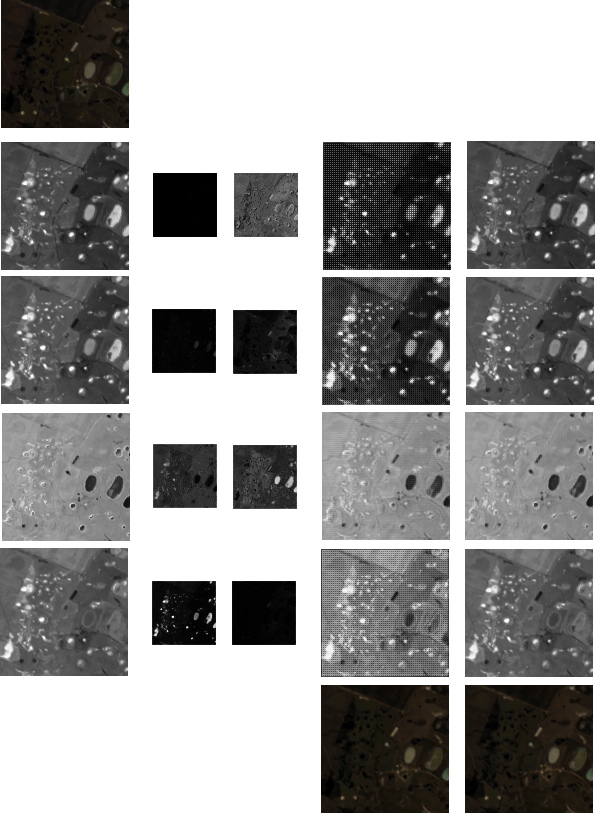
\includegraphics[scale=0.6]{img/latents_2.png}
\caption[Latent Representations]{This image shows four of the 13 channels in the latent representation of an image from the HySpecNet-11k dataset for the model \ac{mymodel}-Fast-AllFrozen for the values 1 and 0.7 for the parameter $\lambda$ of the \ac{dualmse} loss function. The input is on the left. Below it is the latent produced by the spectral encoder, which is shared by both models. Following are, in order, the inner latent produced by the spectral encoder for $\lambda=1$, and for  $\lambda=0.7$, the reconstruction of the latent produced by the spatial decoder for $\lambda=1$ and for $\lambda=0.7$. The full image reconstructions are shown at the bottom.}
\label{fig:latentcompare}
\end{figure}

\begin{figure}
\centering
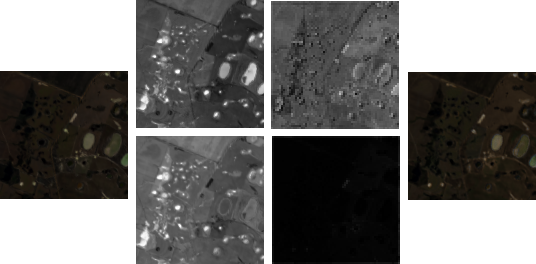
\includegraphics[scale=0.85]{img/innerlatent.png}
\caption[Inner Latent Representations]{Comparison of inner latents for \ac{mymodel}-Fast-AllFrozen with $\lambda=1$ showing partial exploitation of spatial dependencies, especially in the bottom latent. Original image on the left, followed by two latent channels, the corresponding inner latents, and the full image reconstruction.}
\label{fig:innerlatent}
\end{figure}

The best-performing model for this experiment was \textbf{\ac{mymodel}-Fast-EncoderFrozen} with $\lambda=0.5$ with a \ac{psnr} of 45.50 dB and a spectral angle of $3.06 \degree$. The second best model was \textbf{\ac{mymodel}-Fast-AllFrozen} with $\lambda=0.7$ with a \ac{psnr} of 45.31 dB and a spectral angle of $3.22 \degree$.

\section[Analysis of Hyperprior-based Models]{Analysis of Models Using Hyperprior-based Spatial Compression\label{sec:ch5hyperprior}}
\begin{table}
\centering
\caption[Comparison of Hyperprior-based Models]{Comparison of hyperprior-based models. F is the spatial compression/decompression factor in the main encoder/decoder pair.}
\begin{tabular}{|c|c|c|c|c|c|c|}
\hline
Model & F & Loss &$\varphi$ & bpppc & PSNR (dB) & Spectral Angle ($\degree$) \\
\hline\hline
\ac{mymodel}-Attention & 1 & RD & 0.1 & 0.0490 & 21.54 & 21.295 \\
\hline
\ac{mymodel}-Attention & 4 & RD & 0.1 & 0.0012 & 29.67 & 9.547 \\
\hline
\ac{mymodel}-Attention & 16 & RD & 0.1 & 0.0021 & 37.36 & 7.129 \\
\hline
\ac{mymodel}-Attention & 64 & RD & 0.1 & 0.0021 & \textbf{38.99} & \textbf{5.043} \\
\hline
\ac{mymodel}-Attention & 256 & RD & 0.1 & 0.0019 & 36.22 & 6.481 \\
\hline
\ac{mymodel}-Attention & 1 & RD & 5 & 8.3317 & 40.44 & 4.329 \\
\hline
\ac{mymodel}-Attention & 4 & RD & 5 & 0.0199 & 39.32 & 5.159 \\
\hline
\ac{mymodel}-Attention & 16 & RD & 5 & 0.0176 & \textbf{43.65} & \textbf{3.541} \\
\hline
\ac{mymodel}-Attention & 64 & RD & 5 & 0.0151 & 43.39 & 3.697 \\
\hline
\ac{mymodel}-Attention & 256 & RD & 5 & 0.0086 & 41.39 & 4.005 \\
\hline
\ac{mymodel}-Hyperprior & 256 & RD & 0.1 & 0.0082 & 19.30 & 24.56 \\
\hline
\ac{mymodel}-Hyperprior & 256 & MSE & - & 1.071 & 36.80 & 5.79 \\
\hline
\ac{mymodel}-AttUnadjusted & 16 & RD & 0.1 & 0.4327 & 36.58 & 7.503 \\
\hline
\ac{mymodel}-AttUnadjusted & 64 & RD & 0.1 & 0.4198 & 38.819 & 5.109 \\
\hline
\ac{mymodel}-NoQuantization & 4 & MSE & - & 7.6030 & \textbf{48.01} & \textbf{2.816} \\
\hline
\ac{mymodel}-Attention & 4 & MSE & - & 2.9678 & 42.43 & 3.871 \\
\hline
Attention-Based (\citep{cheng_learned_2020}) & 256 & RD & 0.1 & 0.0012 & 33.92 & 8.71 \\
\hline
Scale Hyperprior (\citep{balle_variational_2018}) & 256 & RD & 0.1 & 0.010 & 20.92 & 24.765 \\
\hline
\end{tabular}
\label{fig:hyperpriorcomp}
\end{table}

In this experiment, we compared multiple models using the \ac{mymodel} architecture with a hyperprior-based spatial autoencoder with each other as well as with the hyperprior-based spatial autoencoders outside of \ac{mymodel}. For a detailed explanation of the hyperprior architecture see \autoref{sec3:hyperprior} and for its usage in \ac{mymodel} see \autoref{sec:atthyperprior}. The models \textbf{\ac{mymodel}-Attention} and \textbf{\ac{mymodel}-Hyperprior} (see \autoref{fig:shortnames}) are part of the first category, while Attention-Based and Scale Hyperprior are the respective spatial autoencoders tested separately from the \ac{mymodel} architecture without a reduction in the number of channels beforehand. As usual, we trained \ac{mymodel} approaches by pretraining the spectral autoencoder for 70 epochs. We then froze both the spectral encoder and decoder while training the complete \ac{mymodel} for 50 additional epochs.

The baseline spatial hyperprior-based autoencoder models Attention-Based \citep{cheng_learned_2020} and Scale Hyperprior \citep{balle_variational_2018} compress spatially by a factor of 16 in each spatial dimension in the main encoder. This leads to a total compression factor of F=256 in the main encoder. In order to compare the \ac{mymodel} approaches with the baselines, we also used a spatial compression factor of 256 in the main encoder. We compared these models using $\varphi=0.1$. Our experiments showed that while the model \textbf{\ac{mymodel}-Hyperprior} did not improve upon the baseline, the model \textbf{\ac{mymodel}-Attention} improved upon its baseline by 2.3 dB in \ac{psnr} and $2.22 \degree$ in spectral angle. While it used a slightly higher bitrate of 0.0019 \ac{bpppc} compared to the bitrate of the model Attention-Based of 0.0012 \ac{bpppc}, both models have very low bitrates. For this reason, we focused on decreasing the distortion to achieve closer values to the non-hyperprior-based models while keeping a low bitrate. Furthermore, the attention-based hyperprior performed significantly better than the simple hyperprior-based model. This shows that the inclusion of self-attention modules as well as the context model significantly improves compression performance for a hyperprior-based hyperspectral image compression model. For this reason, we used the model \textbf{\ac{mymodel}-Attention} for the following experiments.

We first modified the model by changing the spatial compression factor in the main encoder. Since the arithmetic coder compressed data losslessly, the quantized output of the main encoder is the direct input to the main decoder, which produces the reconstruction of the input. If we can reduce the loss of information in the spatial encoder, this could therefore reduce the amount of distortion present in the reconstruction. However, simply reducing the compression factor in the main part of the model without modifying the hyperprior autoencoder would increase the size of the bottleneck in the hyperprior autoencoder, therefore increasing the amount of side information that needs to be transmitted. Since the \ac{rd} loss function tries to minimize bitrate, this can also lead to an increase in distortion. We therefore adjusted the spatial compression factor in the hyperprior autoencoder such that the size of the bottleneck in the hyperprior autoencoder is constant. We verified that this approach leads to both a lower distortion and a significantly lower bitrate for the spatial compression factors F=64 and F=16 with $\varphi=0.1$. The model without adjusting the hyperprior autoencoder is the model \textbf{\ac{mymodel}-AttUnadjusted}. For F=16 the adjusted model achieves 2.41 dB \ac{psnr} more with a bitrate that is lower by a factor of $\frac{0.4327}{0.0021} \approx 206$. Additionally, we tested the models with $\varphi=5$ and a selection of models using \ac{mse} loss. As explained in \autoref{sec:ch5ratedistortion}, \ac{mse} loss corresponds to the limit of \ac{mse} loss for $\varphi\rightarrow\infty$. We can therefore use \ac{mse} loss to find a lower bound for the possible amount of distortion achievable with a specific model using \ac{rd} loss. In this way, we show that the model \textbf{\ac{mymodel}-Hyperprior} performs worse than \textbf{\ac{mymodel}-Attention} independent of the value of $\varphi$ by showing that \textbf{\ac{mymodel}-Hyperprior} trained using \ac{mse} loss achieves 36.80 dB \ac{psnr} and a spectral angle of $5.79 \degree$, while \textbf{\ac{mymodel}-Attention} using the same spatial compression factor achieves a \ac{psnr} of 41.39 dB and a spectral angle of $4.005 \degree$ for $\varphi=5$.

The results of the experiments showed that the model \textbf{\ac{mymodel}-Attention} achieves the lowest distortion for spatial compression factors between F=16 and F=64 on the HySpecNet-11k dataset. For $\varphi=0.1$ the lowest distortion of 38.99 dB \ac{psnr} and a spectral angle of $5.043 \degree$ is achieved with a bitrate of 0.0021 \ac{bpppc} for F=64. For $\varphi=5$ the lowest distortion is 43.65 dB \ac{psnr} and a spectral angle of $3.541 \degree$ and is achieved with F=16 with a bitrate of 0.0176 \ac{bpppc}. While F=256 achieves slightly lower bitrates, this also increases distortion significantly. F = 4 results in significantly higher distortion without a significant decrease in bitrate, while F = 1 both increases bitrate and distortion. With regard to the value of $\varphi$, a higher value of $\varphi$ increases bitrate and distortion, as expected. The optimal value of $\varphi$ therefore depends on the desired target bitrate or distortion. 

Additionally, we performed an experiment to test the effect of the quantization step on distortion in the reconstruction in hyperprior-based compression models. \textbf{\ac{mymodel}-NoQuantization} uses the same main autoencoder as the model \textbf{\ac{mymodel}-Attention}. However, it does not use an arithmetic coder or a hyperprior autoencoder in general. Additionally, it does not perform the quantization necessary for a hyperprior model. We compare this model with \textbf{\ac{mymodel}-Attention} also using F=4, trained with \ac{mse} loss. Since the model does not optimize for bitrate in this case and the arithmetic coder is lossless, the only difference between these models pertaining to distortion is the quantization step. \textbf{\ac{mymodel}-NoQuantization} achieves a \ac{psnr} of 48.01 dB which is an improvement of 5.58 dB over the other model. This shows that the quantization step does increase the distortion of hyperprior-based models significantly.

\section[Analysis of Kernel Size Change]{Analysis of Kernel Size Change in 2D CNN-based Spatial Autoencoder}
\begin{table}
\centering
\caption[Kernel Size Comparison For Spatial Autoencoder]{Comparison of different kernel sizes for the spatial autoencoder and per-channel spatial autoencoder with the baseline model. For all models, the spectral encoder is frozen after pretraining and $\lambda = 0.5$.}
\begin{tabular}{|c|c|c|c|}
\hline
Kernel Size & Per Channel? & PSNR (dB) & Spectral Angle ($\degree$) \\
\hline\hline
3 & No & \textbf{45.50} & \textbf{3.06} \\
\hline
5 & No & 43.72 & 3.30 \\
\hline
7 & No & 42.59 & 3.58 \\
\hline
3 & Yes & 42.33 & 3.30 \\
\hline
\end{tabular}
\label{fig:kernelgroups}
\end{table}

To improve the number of spatial dependencies exploited by the \ac{twod} \ac{cnn}-based spatial autoencoder as part of \ac{mymodel}, we experimented with changing the kernel sizes of the convolutional layers of the spatial autoencoder from three to the higher values five and seven. These experiments were performed using the model \textbf{\ac{mymodel}-Fast-EncoderFrozen} with $\lambda=0.5$. However, as seen in \autoref{fig:kernelgroups}, this did not improve either \ac{psnr} or spectral angle. The highest metrics were achieved by the base model using a kernel size of three with 45.50 dB and a spectral angle of $3.06 \degree$. The model using a kernel size of five achieved a lower \ac{psnr} of 43.72 dB and a higher spectral angle of $3.30 \degree$, the model using a kernel size of seven resulted in the lowest \ac{psnr} of 42.59 dB and the lowest spectral angle with $3.58 \degree$. We therefore conclude that a low kernel size of three is optimal for the \ac{cnn}-based spatial autoencoder.

\section[Analysis of Per-Channel Autoencoder]{Analysis of Per-Channel 2D CNN-based Spatial Autoencoder}
On the HySpecNet-11k dataset, the \ac{jpeg} 2000 baseline performed surprisingly well. \Ac{jpeg} 2000 is executed per channel, therefore performing only spatial compression on 202 single-channel images. However, the \ac{twod} \ac{cnn}-based spatial autoencoder uses the same filters to compress all channels in the bottleneck of the spectral autoencoder. We theorized that the differences between the latent channels might be too large to be appropriately captured using the same filters. 

To test this thesis, we modified the \ac{twod} \ac{cnn}-based spatial autoencoder to use a separate set of filters for each channel in the latent. Since this multiplies the number of parameters by the number of latent channels, we reduced the number of filters per channel. For the layers which originally had 256 filters, the modified model only uses 32 filters. For the layers that originally had 512 filters, the modified model uses 64 filters. The reduction in the number of filters is not only appropriate to reduce the number of parameters for the model, but it follows also from the fact that fewer parameters are required for a convolutional layer that captures dependencies for a single channel than a convolutional layer that captures dependencies for multiple channels simultaneously. In total, the number of parameters in the spatial encoder after the reduction in the number of filters rises by 49.3 \% from 50,849,818 to 75,928,346 parameters. We tested the modified model using the model \textbf{\ac{mymodel}-Fast-EncoderFrozen} with $\lambda=0.5$. However, the modification did not significantly change the performance of \ac{mymodel} with regard to the metrics \ac{psnr} or the spectral angle as seen in \autoref{fig:kernelgroups}. 

\section{Rate Distortion Comparison\label{sec:ch5heur}}

\begin{figure}[!ht]
\centering
\pgfplotstableread[col sep=semicolon,]{graphs/bitratecomp.csv}\datatable
\begin{tikzpicture}
\begin{semilogxaxis}[
	log ticks with fixed point,
	grid=both,
    width=\textwidth,
    height=10cm,
    xmin=0.05,
    xtick={0,0.05,0.1,0.25,0.5,1,2,4,8},
    %legend style={at={(0.98,0.05)},anchor=south east},
    legend cell align=left,
    legend columns=3,
    legend style={at={(0.5,-0.2)},anchor=north},
    %legend to name={bitratecomplegend},
    ylabel={PSNR (dB)},
    xlabel={Bits per Pixel per Channel (bpppc)},
	cycle list name=color list,
	log basis x = 10,
	every axis plot/.append style={mark=o} % set options for all plots]
	]
    
    \addplot+ table [x={bpppc}, y={psnr}, 
    restrict expr to domain={\thisrow{model_id}}{2:2}]{\datatable};
    \addlegendentry{\ac{mymodel}-Fast-NF}
    
    \addplot+ table [x={bpppc}, y={psnr}, 
    restrict expr to domain={\thisrow{model_id}}{9:9}]{\datatable};
    \addlegendentry{\ac{mymodel}-Fast-AF}
    
    \addplot+ table [x={bpppc}, y={psnr}, 
    restrict expr to domain={\thisrow{model_id}}{10:10}]{\datatable};
    \addlegendentry{\ac{mymodel}-Fast-EF}
    
    \addplot+ table [x={bpppc}, y={psnr}, 
    restrict expr to domain={\thisrow{model_id}}{3:3}]{\datatable};
    \addlegendentry{Conv1D}
    
    \addplot+ table [x={bpppc}, y={psnr}, 
    restrict expr to domain={\thisrow{model_id}}{4:4}]{\datatable};
    \addlegendentry{\ac{mymodel}}
    
    \addplot+ table [x={bpppc}, y={psnr}, 
    restrict expr to domain={\thisrow{model_id}}{5:5}]{\datatable};
    \addlegendentry{FastConv1D}
    
    \addplot+ table [x={for_combined}, y={psnr}, 
    restrict expr to domain={\thisrow{model_id}}{11:11}]{\datatable};
    \addlegendentry{\ac{mymodel}-Attention}
    
    \addplot+ table [x={bpppc}, y={psnr}, 
    restrict expr to domain={\thisrow{model_id}}{12:12}]{\datatable};
    \addlegendentry{Conv2D}
    
    \addplot+ table [x={bpppc}, y={psnr}, 
    restrict expr to domain={\thisrow{model_id}}{13:13}]{\datatable};
    \addlegendentry{Spectral-VAE}
    
	\addplot+ table [x={bpppc}, y={psnr}, 
    restrict expr to domain={\thisrow{model_id}}{0:0}]{\datatable};
    \addlegendentry{Cubic Interpolation}
    
    \addplot+ table [x={bpppc}, y={psnr}, 
    restrict expr to domain={\thisrow{model_id}}{1:1}]{\datatable};
    \addlegendentry{Linear Interpolation}    
    
    \addplot+ table [x={bpppc}, y={psnr}, 
    restrict expr to domain={\thisrow{model_id}}{8:8}]{\datatable};
    \addlegendentry{JPEG2000}
    
    \node at (axis cs:0.07,43.4) {0.017};
\end{semilogxaxis}
\end{tikzpicture}
%\ref{bitratecomplegend}
\caption[Rate Distortion Plot]{Rate distortion plot showing PSNR for different bitrates for multiple model types.}
\label{fig:ratedistortion}
\end{figure}

Since the distortion produced by a lossy compression method depends on the compression rate \citep{berger_rate-distortion_2003}, we compared the different model architectures used in this thesis for multiple bitrates. We compare all model types listed in \autoref{fig:shortnames} as well as multiple baselines. The models \textbf{Conv1D}, \textbf{FastConv1D} and \textbf{Spectral-VAE} were trained for 70 epochs. The models \textbf{\ac{mymodel}}, \textbf{\ac{mymodel}-Fast} and \textbf{\ac{mymodel}-Attention} were trained for 50 epochs using the corresponding pre-trained spectral autoencoder. The model \textbf{Conv2D} was also trained for 50 epochs. For the model \textbf{\ac{mymodel}-Fast}, three variations were compared. For \textbf{\ac{mymodel}-Fast-NF}, the model is trained without freezing either the spectral encoder or decoder after pretraining, for \textbf{\ac{mymodel}-Fast-EF}, the spectral encoder is frozen after pretraining and for \textbf{\ac{mymodel}-Fast-AF}, the spectral encoder and decoder are frozen after pretraining. While the differences between these options were already discussed for a fixed bitrate of 0.5 bpppc in \autoref{sec:ch5dualmse}, they are also included in this experiment because of the surprising result that freezing the spectral encoder becomes significantly more important for lower bitrates, as discussed below in this section. The model \textbf{\ac{mymodel}-Fast-NF} uses \ac{dualmse} loss with $\lambda=0.5$, the models \textbf{\ac{mymodel}-Fast-EF} and \textbf{\ac{mymodel}-Fast-AF} use $\lambda=1$. For the models \textbf{\ac{mymodel}} and \textbf{\ac{mymodel}-Attention}, the best-performing options were used. For \textbf{\ac{mymodel}}, this is \textbf{EncoderFrozen} with $\lambda=0.5$ and for \textbf{\ac{mymodel}-Attention} this is \textbf{AllFrozen} with $\lambda=1$. The models \textbf{\ac{mymodel}} and \textbf{\ac{mymodel}-Fast} use a spatial compression factor of 4. The highest tested bitrate for such a model is therefore $1/4$ of the highest tested bitrate for the models \textbf{Conv1D} and \textbf{FastConv1D}.

Multiple baselines were used to quantify the performance of the models. The first two baselines, \textbf{Linear Interpolation} and \textbf{Cubic Interpolation} perform simple spectral interpolation. For compression using these methods, a given number of equidistant spectral channels are retained and all others are discarded. For decompression, the original channels are then restored using either linear or cubic interpolation. The first and last channels are always retained, since otherwise restoration of all channels would be impossible without extrapolating values. These methods were used as baselines because of the assumption that nearby spectral channels have similar values for the same pixel since they capture wavelengths that are close together. The third baseline used was \ac{jpeg} 2000, which was applied per channel. The tested quality settings for \ac{jpeg} 2000 were 1, 2, 3, 4, 5, 10, 15 and 20. We also consider \textbf{Conv1D} a baseline, since it is based on the model proposed in Kuester et al. \citep{kuester_1d-convolutional_2021,kuester_transferability_2022}.

The results show that the model \textbf{Spectral-VAE} is not successful in performing hyperspectral image compression by reducing the number of spectral channels. This is not surprising since the \ac{vae} architecture in \ac{rgb} image compression is also not commonly applied directly but rather through using a hyperprior architecture. A hyperprior-based spectral autoencoder is tested and discussed in \autoref{sec:ch5hyperprior}. All other tested models outperform the interpolation-based baselines, showing that the spectral dependencies are too complex to be captured using only interpolation.

In comparison with the \ac{jpeg} 2000 baseline and the models using the \ac{mymodel} architecture, the purely spectral compression methods \textbf{Conv1D} and \textbf{FastConv1D} perform best for bitrates close to 0.5 \ac{bpppc}. The model \textbf{Conv1D} outperforms \ac{jpeg} 2000 for the bitrate 0.63 \ac{bpppc}. Note that different model types can be tested for slightly different bitrates because of different padding strategies. Additionally, \ac{jpeg} 2000 can only be set to a fixed number of different quality settings and therefore does not allow for setting a specific bitrate. The model \textbf{FastConv1D} has a higher \ac{psnr} than \ac{jpeg} 2000 for bitrates from 0.31 to 0.47 \ac{bpppc}. These correspond to two and respectively three channels in the latent representation. For higher bitrates, \ac{jpeg} 2000 outperforms the spectral encoding methods. Further, the model \textbf{Conv1D} has a lower limit on the number of spectral channels in the latent dimensions, below which distortion strongly increases. This point is at 2 latent channels, which corresponds to a bitrate of 0.31 \ac{bpppc}, where it achieves a \ac{psnr} of 20.40 dB, while for 4 latent channels, the model achieves 43.63 dB for a bitrate of 0.63 \ac{bpppc}.

The \ac{mymodel} architecture outperforms all baselines and other compared models for bitrates at or below 0.5 \ac{bpppc}. The model \textbf{\ac{mymodel}} has a \ac{psnr} of 43.48 dB when using 13 latent channels which results in a bitrate of 0.51 \ac{bpppc}. For 26 latent channels, the model does not significantly improve, achieving a \ac{psnr} of 43.85 dB with a bitrate of 1.03 \ac{bpppc}, which is worse than \textbf{Conv1D}, \textbf{FastConv1D} and \ac{jpeg} 2000 for similar bitrates. This is expected since the idea of the \ac{mymodel} architecture is to first reduce the number of spectral channels in order to be able to use spatial compression methods that work best for images with a low number of spectral channels such as \ac{rgb} or multispectral images. This is also illustrated by the model \textbf{Conv2D}, which shows the \ac{twod} \ac{cnn}-based spatial autoencoder directly applied to the hyperspectral data. This model only achieves a \ac{psnr} of 35.734 dB for a bitrate of 0.51 \ac{bpppc}, which shows that a reduction in the number of channels can strongly improve the performance of spatial compression methods. The effect is further shown by the model \textbf{AttentionHyperprior}, which uses the spatial autoencoder of the \textbf{\ac{mymodel}-Attention} model without first reducing the number of spectral channels, achieving a much lower \ac{psnr} of 33.92 dB. The model \textbf{\ac{mymodel}-Fast-AF} achieves the highest \ac{psnr} of all compared models, 44.59 dB, for the bitrate 0.51. For the bitrates 0.23 \ac{bpppc} and 0.12 \ac{bpppc}, it is the second best model behind \textbf{\ac{mymodel}-Attention} with \acp{psnr} of 42.35 and 38.98 respectively. However, the model \textbf{\ac{mymodel}-Fast-NF} performs much worse for the bitrate $0.12$ with only a \ac{psnr} of 20.44 dB. It follows that freezing the spectral encoder is important when training for very low bitrates.

For all bitrates below 0.25, the highest \ac{psnr} is achieved by the model \textbf{\ac{mymodel}-Attention}. Additionally, this distortion is achieved with a much lower bitrate than in other models with similar \ac{psnr} values. In comparison with the second model with the second lowest bitrate for similar distortion, \textbf{\ac{mymodel}-Fast-AF}, the compression rate differs by a factor of $0.24/0.017=14.11$. We conclude that for the HySpecNet-11k the \textbf{\ac{mymodel}-Attention} model is optimal in order to achieve bitrates $<0.25$ \ac{bpppc}, while the \textbf{\ac{mymodel}-Fast} model can achieve slightly lower distortion for bitrates $\approx 0.5$ \ac{bpppc}. Additionally, the results show that the \ac{mymodel} approach improves upon the purely spectral compression methods and purely spatial compression for bitrates lower than 1 \ac{bpppc}. 






